\subsection{图的存储结构}

\subsubsection{邻接矩阵}
\begin{frame}\ft{\subsubsecname}
由于图是有顶点和边或弧两部分组成的,可以考虑分两个结构分别来存储。
\begin{itemize}
\item[(1)] 顶点不分大小、主次,可用一个一维数组来存储。
\item[(2)] 边或弧为顶点与顶点之间的关系,可用一个二维数组来存储。\end{itemize}
此即邻接矩阵的存储方案。
\end{frame}

\begin{frame}\ft{\subsecname}
\begin{dingyi}[邻接矩阵]
\tf图的邻接矩阵(Adjacency matrix)存储方式是用两个数组来表示图。一个一维数组存储图中顶点信息,一个二维数组(称为邻接矩阵)存储图中的边或弧的信息。
\end{dingyi}
设图$G$有$n$个顶点,则邻接矩阵为一个$n\times n$的方阵,定义为
$$
e[i][j]=\left\{
\begin{array}{ll}
1,& \mbox{\tf if $(v_i,v_j)\in E$ or $<v_i,v_j>\in E$}, \\[0.05in]
0,& \mbox{\tf otherwise}.
\end{array}
\right.
$$
\end{frame}

\begin{frame}\ft{\subsecname}
\begin{figure} 
\centering
\begin{tikzpicture}[scale=1.5,node distance=3cm,semithick,inner sep=1pt,bend angle=45,auto]
%\draw[help lines] (-1,-1) grid (5,3);
\node[state]   (v0) at (30:1)  {$v_0$};
\node[state]   (v1) at (0:0)   {$v_1$};
\node[state]   (v2) at (-40:1) {$v_2$};
\node[state]   (v3) at (-5:1.8)  {$v_3$};
\path
(v0) edge (v1)
     edge (v2)   
     edge (v3)
(v1) edge (v2)
(v2) edge (v3);   

\matrix (am) at (3,0) [matrix of math nodes,left delimiter=(,right delimiter=),row sep=10pt,column sep=10pt,right] 
  {
    0 & 1 & 1 & 1\\
    1 & 0 & 1 & 0\\
    1 & 1 & 0 & 1\\
    1 & 0 & 1 & 0\\
  };
  \node at (am-1-1) [above=10pt] {$v_0$}; 
  \node at (am-1-2) [above=10pt] {$v_1$};       
  \node at (am-1-3) [above=10pt] {$v_2$};       
  \node at (am-1-4) [above=10pt] {$v_3$};
  \node at (am-1-1) [left=15pt] {$v_0$}; 
  \node at (am-2-1) [left=15pt] {$v_1$};       
  \node at (am-3-1) [left=15pt] {$v_2$};       
  \node at (am-4-1) [left=15pt] {$v_3$};             

%\matrix (v) at (3,2) [matrix of math nodes,left delimiter=(,right delimiter=),row sep=10pt,column sep=10pt,right]{
%  v_0 & v_1 & v_2 & v_3\\
%};


\end{tikzpicture}

\caption{无向图的邻接矩阵为对称矩阵}
\end{figure}
\end{frame}

\begin{frame}\ft{\subsecname}
%有了邻接矩阵,可以很容易地得到无向图中的信息。\\[0.03in]
\begin{itemize}
\item[1] 可以很容易地判定任意两顶点是否有边。\\[0.1in]
\item[2] 顶点$v_i$的度等于邻接矩阵中第$i$行的元素之和。\\[0.1in]
\item[3] 欲求顶点$v_i$的所有邻接点,只需扫描邻接矩阵的第$i$行,若$e[i][j]=1$,则$v_j$为其邻接点。

\end{itemize}•
\end{frame}

\begin{frame}\ft{\subsecname}
\begin{figure}
\centering
\begin{tikzpicture}[scale=1.5,->,>=stealth',node distance=3cm,semithick,inner sep=1pt,bend angle=45,auto]
%\draw[help lines] (-1,-1) grid (5,3);
\node[state]   (v0) at (30:1)  {$v_0$};
\node[state]   (v1) at (0:0)   {$v_1$};
\node[state]   (v2) at (-40:1) {$v_2$};
\node[state]   (v3) at (-5:1.8)  {$v_3$};
\path
(v0) edge (v3)
(v1) edge (v0)
     edge[bend right=10] (v2)   
(v2) edge[bend right=10] (v1)
     edge (v0);   

\matrix (am) at (3,0) [matrix of math nodes,left delimiter=(,right delimiter=),row sep=10pt,column sep=10pt,right] 
  {
    0 & 0 & 0 & 1\\
    1 & 0 & 1 & 0\\
    1 & 1 & 0 & 0\\
    0 & 0 & 0 & 0\\
  };
  \node at (am-1-1) [above=10pt] {$v_0$}; 
  \node at (am-1-2) [above=10pt] {$v_1$};       
  \node at (am-1-3) [above=10pt] {$v_2$};       
  \node at (am-1-4) [above=10pt] {$v_3$};
  \node at (am-1-1) [left=15pt] {$v_0$}; 
  \node at (am-2-1) [left=15pt] {$v_1$};       
  \node at (am-3-1) [left=15pt] {$v_2$};       
  \node at (am-4-1) [left=15pt] {$v_3$};             

\matrix (v) at (3,2) [matrix of math nodes,left delimiter=(,right delimiter=),row sep=10pt,column sep=10pt,right]{
  v_0 & v_1 & v_2 & v_3\\
};


\end{tikzpicture}

\caption{有向图的邻接矩阵不是对称矩阵}
\end{figure}
\end{frame}


\begin{frame}\ft{\subsecname}
%有了邻接矩阵,可以很容易地得到图中的信息。\\[0.03in]
\begin{itemize}
\item[1] 顶点$v_i$的入度等于邻接矩阵中第$i$列的元素之和;顶点$v_i$的出度等于邻接矩阵中第$i$行的元素之和。\\[0.1in]
\item[2] 欲判断顶点$v_i$到$v_j$是否有弧,只需查找$e[i][j]$是否为1。\\[0.1in]
\item[3] 欲求顶点$v_i$的所有邻接点,只需扫描邻接矩阵的第$i$行,若$e[i][j]=1$,则$v_j$为其邻接点。
\end{itemize}
\end{frame}

\begin{frame}\ft{\subsecname}
设图$G$是网,有$n$个顶点,则邻接矩阵是一个$n\times n$的方阵,定义为
$$
e[i][j]=\left\{
\begin{array}{ll}
w_{ij}, & \mbox{\tf if $(v_i,v_j)\in E$ or $<v_i,v_j>\in E$}, \\[0.05in]
0,& \mbox{if i=j}\\[0.05in]
\infty,&\mbox{\tf otherwise}.
\end{array}
\right.
$$
\end{frame}


\begin{frame}\ft{\subsecname}
\begin{figure}
\centering
\begin{tikzpicture}[scale=1.5,->,>=stealth',node distance=3cm,semithick,inner sep=1pt,bend angle=45,auto]
%\draw[help lines] (-1,-1) grid (5,3);
\node[state]   (v0) at (90:1)  {$v_0$};
\node[state]   (v1) at (90+72:1)   {$v_1$};
\node[state]   (v2) at (90+2*72:1) {$v_2$};
\node[state]   (v3) at (90+3*72:1)  {$v_3$};
\node[state]   (v4) at (90+4*72:1)  {$v_4$};
\path
(v0) edge node{6} (v4)
(v1) edge node{9} (v0)
     edge node{3} (v2)   
(v2) edge node{2} (v0)
     edge node{5} (v3)
(v3) edge node{1} (v4);   

\matrix (am) at (3,0) [matrix of math nodes,left delimiter=(,right delimiter=),row sep=10pt,column sep=10pt,right] 
  {
    0 & \infty & \infty & \infty & 6\\
    9 & 0 & 3 & \infty & \infty \\
    2 & \infty & 0 & 5 & \infty \\
    \infty & \infty & \infty & 0 & 1\\
    \infty & \infty & \infty & \infty & 1\\
  };
  \node at (am-1-1) [above=10pt] {$v_0$}; 
  \node at (am-1-2) [above=10pt] {$v_1$};       
  \node at (am-1-3) [above=10pt] {$v_2$};       
  \node at (am-1-4) [above=10pt] {$v_3$};
  \node at (am-1-5) [above=10pt] {$v_4$};
  \node at (am-1-1) [left=18pt] {$v_0$}; 
  \node at (am-2-1) [left=18pt] {$v_1$};       
  \node at (am-3-1) [left=18pt] {$v_2$};       
  \node at (am-4-1) [left=18pt] {$v_3$};             
  \node at (am-5-1) [left=18pt] {$v_4$};             
\matrix (v) at (3,2) [matrix of math nodes,left delimiter=(,right delimiter=),row sep=10pt,column sep=10pt,right]{
  v_0 & v_1 & v_2 & v_3 & v_4\\
};


\end{tikzpicture}

\caption{网的邻接矩阵}
\end{figure}

\end{frame}


\begin{frame}\ft{\subsecname}
\lstinputlisting[
title=\tf adjmatrix.h,
language=C,
frame=tb,
]{Chapters/Ch06/Code/adjmatrix/adjmatrix.h}
\end{frame}

\begin{frame}\ft{\subsecname}
\lstinputlisting[
title=\tf adjmatrix.h,
language=C,
frame=tb,
]{Chapters/Ch06/Code/adjmatrix/adjmatrix.c}
\end{frame}



\subsubsection{邻接表}

\begin{frame}\ft{\subsubsecname}
\begin{figure}
\centering
\begin{tikzpicture}[scale=1.5,->,>=stealth',node distance=3cm,semithick,inner sep=1pt,bend angle=45,auto]
%\draw[help lines] (-1,-1) grid (5,3);
\node[state]   (v0) at (90:1)  {$v_0$};
\node[state]   (v1) at (90+72:1)   {$v_1$};
\node[state]   (v2) at (90+2*72:1) {$v_2$};
\node[state]   (v3) at (90+3*72:1)  {$v_3$};
\node[state]   (v4) at (90+4*72:1)  {$v_4$};
\path

(v1) edge node{9} (v0);   

\matrix (am) at (3,0) [matrix of math nodes,left delimiter=(,right delimiter=),row sep=10pt,column sep=10pt,right] 
  {
    0 & \infty & \infty & \infty & \infty\\
    9 & 0 & \infty & \infty & \infty \\
    \infty & \infty & 0 & \infty & \infty \\
    \infty & \infty & \infty & 0 & \infty\\
    \infty & \infty & \infty & \infty & \infty\\
  };
  \node at (am-1-1) [above=10pt] {$v_0$}; 
  \node at (am-1-2) [above=10pt] {$v_1$};       
  \node at (am-1-3) [above=10pt] {$v_2$};       
  \node at (am-1-4) [above=10pt] {$v_3$};
  \node at (am-1-5) [above=10pt] {$v_4$};
  \node at (am-1-1) [left=18pt] {$v_0$}; 
  \node at (am-2-1) [left=18pt] {$v_1$};       
  \node at (am-3-1) [left=18pt] {$v_2$};       
  \node at (am-4-1) [left=18pt] {$v_3$};             
  \node at (am-5-1) [left=18pt] {$v_4$};             
\matrix (v) at (3,2) [matrix of math nodes,left delimiter=(,right delimiter=),row sep=10pt,column sep=10pt,right]{
  v_0 & v_1 & v_2 & v_3 & v_4\\
};


\end{tikzpicture}

\end{figure}
\end{frame}


\begin{frame}\ft{\subsecname}
\begin{dingyi}
数组与链表结合的存储方法称为邻接表。
\end{dingyi}


\begin{itemize}
\item
顶点用一维数组存储。数组中每个元素还需存储指向第一个邻接点的指针,以便于查找该顶点的边信息。 \\[0.1in]
\item
每个顶点$v_i$的所有邻接点构成一个线性表。由于邻接点个数不定,故以单链表存储,无向图称为$v_i$的边表,有向图则称为$v_i$作为弧尾的出边表。
\end{itemize}

\end{frame}


\begin{frame}\ft{\subsecname}
\begin{figure}
\centering
\begin{tikzpicture}[scale=1.5,node distance=3cm,semithick,inner sep=1pt,bend angle=45,auto]
%\draw[help lines] (0,-1) grid (7,3);
\node[state]   (v0) at (30:1)  {$v_0$};
\node[state]   (v1) at (0:0)   {$v_1$};
\node[state]   (v2) at (-40:1) {$v_2$};
\node[state]   (v3) at (-5:1.8)  {$v_3$};
\path
(v0) edge (v1)
     edge (v2)   
     edge (v3)
(v1) edge (v2)
(v2) edge (v3);   

\def\dd{0.5}
\foreach \i in {0,1,2,3}{
\draw (2.2,\i*\dd) rectangle(3.2,\i*\dd+\dd);
\draw (2.8,\i*\dd)-- (2.8,\i*\dd+\dd);
\node at (2.45,-\i*\dd+3.5*\dd){$v_\i$};
}
\node at (2.45,2) [above]{\tf data};
\node at (2.95,2) [above=10pt]{\tf firstedge};


\def\dd{0.5}
\foreach \i in {0,1,2,3}{
\draw[->,>=latex'] (2.95,\i*\dd+0.5*\dd)--(3.4,\i*\dd+0.5*\dd);
\draw (3.4,\i*\dd) rectangle(4.4,\i*\dd+\dd);
\draw (3.9,\i*\dd)-- (3.9,\i*\dd+\dd);
\ifthenelse{\i=0}{
\node at (3.65,-\i*\dd+3.5*\dd){$1$};
}{
\node at (3.65,-\i*\dd+3.5*\dd){$0$};
}
}

\node at (3.65,2) [above]{\tf adjvex};
\node at (4.15,2) [above=10pt]{\tf next};

\def\dd{0.5}
\foreach \i in {0,1,2,3}{
\draw[->,>=latex'] (4.15,\i*\dd+0.5*\dd)--(4.6,\i*\dd+0.5*\dd);
\draw (4.6,\i*\dd) rectangle(5.6,\i*\dd+\dd);
\draw (5.1,\i*\dd)-- (5.1,\i*\dd+\dd);
\ifthenelse{\i=2}{
\node at (4.85,-\i*\dd+3.5*\dd){$1$};
}{
\node at (4.85,-\i*\dd+3.5*\dd){$2$};
}
}


\def\dd{0.5}
\foreach \i in {1,3}{
\draw[->,>=latex'] (5.35,\i*\dd+0.5*\dd)--(5.8,\i*\dd+0.5*\dd);
\draw (5.8,\i*\dd) rectangle(6.8,\i*\dd+\dd);
\draw (6.3,\i*\dd)-- (6.3,\i*\dd+\dd);
\node at (6.05,\i*\dd+0.5*\dd){$3$};
}






\end{tikzpicture}

\end{figure}

\end{frame}


\begin{frame}\ft{\subsecname}
\begin{figure}
\centering
\begin{tikzpicture}[scale=1.5,node distance=3cm,semithick,inner sep=1pt,bend angle=45,auto]
%\draw[help lines] (0,-1) grid (7,3);
\node[state]   (v0) at (30:1)  {$v_0$};
\node[state]   (v1) at (0:0)   {$v_1$};
\node[state]   (v2) at (-40:1) {$v_2$};
\node[state]   (v3) at (-5:1.8)  {$v_3$};
\path
(v0) edge[->,>=latex'] (v3)
(v1) edge[->,>=latex']  (v0)
       edge[->,>=latex',bend right=10] (v2)
(v2) edge[->,>=latex',bend right=10] (v1)
       edge[->,>=latex']  (v0);   

\def\dd{0.5}
\foreach \i in {0,1,2,3}{
\draw (2.2,\i*\dd) rectangle(3.2,\i*\dd+\dd);
\draw (2.8,\i*\dd)-- (2.8,\i*\dd+\dd);
\node at (2.45,-\i*\dd+3.5*\dd){$v_\i$};
}
\node at (2.45,2) [above]{\tf data};
\node at (2.95,2) [above=10pt]{\tf firstedge};


\def\dd{0.5}
\foreach \i in {1,2,3}{
\draw[->,>=latex'] (2.95,\i*\dd+0.5*\dd)--(3.4,\i*\dd+0.5*\dd);
\draw (3.4,\i*\dd) rectangle(4.4,\i*\dd+\dd);
\draw (3.9,\i*\dd)-- (3.9,\i*\dd+\dd);
\ifthenelse{\i=3}{
\node at (3.65,\i*\dd+0.5*\dd){$3$};
}{
\node at (3.65,\i*\dd+0.5*\dd){$0$};
}
}

\node at (3.65,2) [above]{\tf adjvex};
\node at (4.15,2) [above=10pt]{\tf next};

\def\dd{0.5}
\foreach \i in {1,2}{
\draw[->,>=latex'] (4.15,\i*\dd+0.5*\dd)--(4.6,\i*\dd+0.5*\dd);
\draw (4.6,\i*\dd) rectangle(5.6,\i*\dd+\dd);
\draw (5.1,\i*\dd)-- (5.1,\i*\dd+\dd);
\ifthenelse{\i=2}{
\node at (4.85,\i*\dd+0.5*\dd){$2$};
}{
\node at (4.85,\i*\dd+0.5*\dd){$1$};
}
}




%%%%%%%%%%%

\def\yy{-2.7}


\foreach \i in {0,1,2,3}{
\draw (2.2,\i*\dd+\yy) rectangle(3.2,\i*\dd+\dd+\yy);
\draw (2.8,\i*\dd+\yy)-- (2.8,\i*\dd+\dd+\yy);
\node at (2.45,-\i*\dd+3.5*\dd+\yy){$v_\i$};
}
\node at (2.45,2+\yy) [above]{\tf data};
\node at (2.95,2+\yy) [above=10pt]{\tf firstedge};


\def\dd{0.5}
\foreach \i in {0,1,2,3}{
\draw[->,>=latex'] (2.95,\i*\dd+0.5*\dd+\yy)--(3.4,\i*\dd+0.5*\dd+\yy);
\draw (3.4,\i*\dd+\yy) rectangle(4.4,\i*\dd+\dd+\yy);
\draw (3.9,\i*\dd+\yy)-- (3.9,\i*\dd+\dd+\yy);
\ifthenelse{\i=2}{
\node at (3.65,\i*\dd+0.5*\dd+\yy){$2$};
}{
\ifthenelse{\i=0}{
\node at (3.65,\i*\dd+0.5*\dd+\yy){$0$};
}{
\node at (3.65,\i*\dd+0.5*\dd+\yy){$1$};
}
}
}

\node at (3.65,2+\yy) [above]{\tf adjvex};
\node at (4.15,2+\yy) [above=10pt]{\tf next};

\def\dd{0.5}
\foreach \i in {3}{
\draw[->,>=latex'] (4.15,\i*\dd+0.5*\dd+\yy)--(4.6,\i*\dd+0.5*\dd+\yy);
\draw (4.6,\i*\dd+\yy) rectangle(5.6,\i*\dd+\dd+\yy);
\draw (5.1,\i*\dd+\yy)-- (5.1,\i*\dd+\dd+\yy);
\node at (4.85,\i*\dd+0.5*\dd+\yy){$2$};

}






\end{tikzpicture}

\end{figure}

\end{frame}


\begin{frame}\ft{\subsecname}
\begin{figure}
\centering
\begin{tikzpicture}[scale=1.5,node distance=3cm,semithick,inner sep=1pt,bend angle=45,auto]
%\draw[help lines] (0,-1) grid (7,3);
\node[state]   (v0) at (90:1)  {$v_0$};
\node[state]   (v1) at (90+72:1)   {$v_1$};
\node[state]   (v2) at (90+2*72:1) {$v_2$};
\node[state]   (v3) at (90+3*72:1)  {$v_3$};
\node[state]   (v4) at (90+4*72:1)  {$v_4$};
\path
(v0) edge[->,>=latex'] node{6} (v4)
(v1) edge[->,>=latex'] node{9} (v0)
     edge[->,>=latex'] node{3} (v2)   
(v2) edge[->,>=latex'] node{2} (v0)
     edge[->,>=latex'] node{5} (v3)
(v3) edge[->,>=latex'] node{1} (v4); 

\def\dd{0.5}
\foreach \i in {0,1,2,3,4}{
\draw (2.2,\i*\dd) rectangle(3.2,\i*\dd+\dd);
\draw (2.8,\i*\dd)-- (2.8,\i*\dd+\dd);
\node at (2.45,-\i*\dd+4.5*\dd){$v_\i$};
}
\node at (2.45,2.5) [above]{\tf data};
\node at (2.95,2.5) [above=20pt]{\tf firstedge};


\def\dd{0.5}
\foreach \i in {1,2,3,4}{
\draw[->,>=latex'] (2.95,\i*\dd+0.5*\dd)--(3.4,\i*\dd+0.5*\dd);
\draw (3.4,\i*\dd) rectangle(4.6,\i*\dd+\dd);
\draw (3.8,\i*\dd)-- (3.8,\i*\dd+\dd);
\draw (4.2,\i*\dd)-- (4.2,\i*\dd+\dd);
\ifthenelse{\i=1 \OR \i=4}{
\node at (3.6,\i*\dd+0.5*\dd){$4$};
}{
\node at (3.6,\i*\dd+0.5*\dd){$0$};
}

\ifthenelse{\i=1}{
\node at (4.0,\i*\dd+0.5*\dd){$1$};
}{
\ifthenelse{\i=2}{
\node at (4.0,\i*\dd+0.5*\dd){$2$};
}{
\ifthenelse{\i=3}{
\node at (4.0,\i*\dd+0.5*\dd){$9$};
}{
\node at (4.0,\i*\dd+0.5*\dd){$6$};
}

}
}


}

\node at (3.6,2.5) [above]{\tf adjvtx};
\node at (4.0,2.5) [above=20pt]{\tf weight};
\node at (4.4,2.5) [above]{\tf next};

\def\dd{0.5}
\foreach \i in {2,3}{
\draw[->,>=latex'] (4.4,\i*\dd+0.5*\dd)--(4.8,\i*\dd+0.5*\dd);
\draw (4.8,\i*\dd) rectangle(6.0,\i*\dd+\dd);
\draw (5.2,\i*\dd)-- (5.2,\i*\dd+\dd);
\draw (5.6,\i*\dd)-- (5.6,\i*\dd+\dd);
\ifthenelse{\i=2}{
\node at (5.0,\i*\dd+0.5*\dd){$3$};
}{
\node at (5.0,\i*\dd+0.5*\dd){$2$};
}

\ifthenelse{\i=2}{
\node at (5.4,\i*\dd+0.5*\dd){$5$};
}{
\node at (5.4,\i*\dd+0.5*\dd){$3$};
}

}







\end{tikzpicture}

\end{figure}
\end{frame}


\begin{frame}\ft{\subsecname}
  \lstinputlisting[
    language=C,
    title=\tf adjlist.h,
    numbers=left,
    numberstyle=\tiny,
    frame=tb,
    xleftmargin=3pt,
  ]{Chapters/Ch06/Code/adjlist/adjlist.h}
\end{frame}

\begin{frame}\ft{\subsecname}
  \lstinputlisting[
    language=C,
    title=\tf CreateALGraph.c,
    numbers=left,
    numberstyle=\tiny,
    linerange={3-12},
    frame=tb,
    xleftmargin=3pt,
  ]{Chapters/Ch06/Code/adjlist/adjlist.c}
\end{frame}

\begin{frame}\ft{\subsecname}
  \lstinputlisting[
    language=C,
    title=\tf CreateALGraph.c,
    numbers=left,
    numberstyle=\tiny,
    firstnumber=11,
    linerange={14-27},
    frame=tb,
    xleftmargin=3pt,
  ]{Chapters/Ch06/Code/adjlist/adjlist.c}
\end{frame}


%%%%%%%%%%%%%%%%%%%%%
\subsubsection{十字链表}
%%%%%%%%%%%%%%%%%%%%%
\begin{frame}  
  \begin{figure}
    \centering
    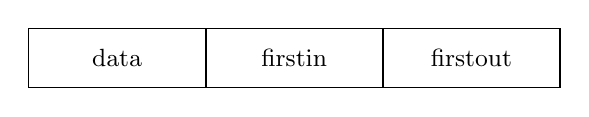
\begin{tikzpicture}[scale=1.5,node distance=3cm,semithick,inner sep=1pt,bend angle=45,auto]
  \draw(0,0)rectangle(4.5,0.5);
  \draw(1.5,0)rectangle(1.5,0.5);
  \draw(3.0,0)rectangle(3.0,0.5);
  \node at(0.75,0.25){\tf \small data};
  \node at(2.25,0.25){\tf \small firstin};
  \node at(3.75,0.25){\tf \small firstout};
\end{tikzpicture}

    \caption{十字链表的顶点表结点结构}    
  \end{figure}  
  \begin{itemize}
  \item \tf firstin:入边表头指针,指向该顶点的入边表中第一个结点\\[0.1in]
  \item \tf firstout:出边表头指针,指向该顶点的出边表中的第一个结点
  \end{itemize}

\end{frame}

\begin{frame}  
  \begin{figure}
    \centering
    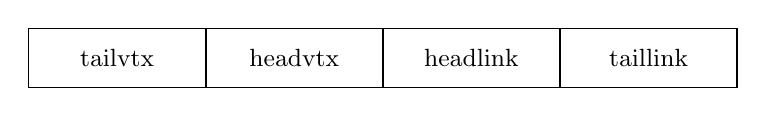
\begin{tikzpicture}[scale=1.5,node distance=3cm,semithick,inner sep=1pt,bend angle=45,auto]
  \draw(0,0)rectangle(6,0.5);
  \draw(1.5,0)rectangle(1.5,0.5);
  \draw(3.0,0)rectangle(3.0,0.5);
  \draw(4.5,0)rectangle(4.5,0.5);
  \node at(0.75,0.25){\tf \small tailvtx};
  \node at(2.25,0.25){\tf \small headvtx};
  \node at(3.75,0.25){\tf \small headlink};
  \node at(5.25,0.25){\tf \small taillink};
\end{tikzpicture}

    \caption{十字链表的边表结点结构}    
  \end{figure}  
  
  \begin{itemize}
  \item \tf tailvtx:弧起点在顶点表的下标 \\[0.1in]
  \item \tf headvtx:弧终点在顶点表中的下标 \\[0.1in]
  \item \tf headlink:入边表指针域,指向终点相同的下一条边 \\[0.1in]
  \item \tf taillink:出边表指针域,指向起点相同的下一条边 \\[0.1in]
  \item \tf 若是网,还可再增加一个weight值来存储权值。
  \end{itemize}
\end{frame}

\begin{frame}\ft{\subsubsecname}
  \begin{figure}
    \centering
    \begin{tikzpicture}[scale=1.5,node distance=3cm,semithick,inner sep=1pt,bend angle=45,auto]
%\draw[help lines] (0,-1) grid (7,3);
\node[state]   (v0) at (30:1)  {$v_0$};
\node[state]   (v1) at (0:0)   {$v_1$};
\node[state]   (v2) at (-40:1) {$v_2$};
\node[state]   (v3) at (-5:1.8)  {$v_3$};
\path
(v0) edge (v1)
     edge (v2)   
     edge (v3)
(v1) edge (v2)
(v2) edge (v3);   

\def\dd{0.5}
\foreach \i in {-2,0,2,4}{
\draw (2.2,\i*\dd) rectangle(3.2,\i*\dd+\dd);
\draw (2.8,\i*\dd)-- (2.8,\i*\dd+\dd);
\node at (2.45,-\i*\dd+3.5*\dd) {$v_\i$};
}
\node at (2.45,2) [above]{\tf data};
\node at (2.95,2) [above=10pt]{\tf firstedge};


\def\dd{0.5}
\foreach \i in {0,1,2,3}{
\draw[->,>=latex'] (2.95,\i*\dd+0.5*\dd)--(3.4,\i*\dd+0.5*\dd);
\draw (3.4,\i*\dd) rectangle(4.4,\i*\dd+\dd);
\draw (3.9,\i*\dd)-- (3.9,\i*\dd+\dd);
\ifthenelse{\i=0}{
\node at (3.65,-\i*\dd+3.5*\dd){$1$};
}{
\node at (3.65,-\i*\dd+3.5*\dd){$0$};
}
}

\node at (3.65,2) [above]{\tf adjvex};
\node at (4.15,2) [above=10pt]{\tf next};

\def\dd{0.5}
\foreach \i in {0,1,2,3}{
\draw[->,>=latex'] (4.15,\i*\dd+0.5*\dd)--(4.6,\i*\dd+0.5*\dd);
\draw (4.6,\i*\dd) rectangle(5.6,\i*\dd+\dd);
\draw (5.1,\i*\dd)-- (5.1,\i*\dd+\dd);
\ifthenelse{\i=2}{
\node at (4.85,-\i*\dd+3.5*\dd){$1$};
}{
\node at (4.85,-\i*\dd+3.5*\dd){$2$};
}
}


\def\dd{0.5}
\foreach \i in {1,3}{
\draw[->,>=latex'] (5.35,\i*\dd+0.5*\dd)--(5.8,\i*\dd+0.5*\dd);
\draw (5.8,\i*\dd) rectangle(6.8,\i*\dd+\dd);
\draw (6.3,\i*\dd)-- (6.3,\i*\dd+\dd);
\node at (6.05,\i*\dd+0.5*\dd){$3$};
}






\end{tikzpicture}

  \end{figure}

\end{frame}


\begin{frame}\ft{\subsubsecname}
  十字链表的好处是把邻接表和逆邻接表整合在了一起,这样既可以容易地找到以$v_i$为尾的弧,也可以容易地找到以$v_i$为头的弧,因而可以容易地求得顶点的出度和入度。在有向图的应用中,十字链表是非常好的数据类型结构。
\end{frame}
